\documentclass[11pt]{article}


\usepackage{fullpage}
\usepackage{graphicx}
\usepackage{amsmath}
\usepackage{amssymb}
\usepackage{amsthm}
\usepackage{fancyvrb}

\newcommand{\myname}{Mehshan Mustafa}

\newenvironment{theorem}[2][Theorem]{\begin{trivlist}
\item[\hskip \labelsep {\bfseries #1}\hskip \labelsep {\bfseries #2.}]}{\end{trivlist}}
\newenvironment{lemma}[2][Lemma]{\begin{trivlist}
\item[\hskip \labelsep {\bfseries #1}\hskip \labelsep {\bfseries #2.}]}{\end{trivlist}}
\newenvironment{exercise}[2][Exercise]{\begin{trivlist}
\item[\hskip \labelsep {\bfseries #1}\hskip \labelsep {\bfseries #2.}]}{\end{trivlist}}
\newenvironment{problem}[2][Problem]{\begin{trivlist}
\item[\hskip \labelsep {\bfseries #1}\hskip \labelsep {\bfseries #2.}]}{\end{trivlist}}
\newenvironment{question}[2][Question]{\begin{trivlist}
\item[\hskip \labelsep {\bfseries #1}\hskip \labelsep {\bfseries #2.}]}{\end{trivlist}}
\newenvironment{corollary}[2][Corollary]{\begin{trivlist}
\item[\hskip \labelsep {\bfseries #1}\hskip \labelsep {\bfseries #2.}]}{\end{trivlist}}
\newenvironment{solution}{\begin{proof}[Solution]}{\end{proof}}
\newenvironment{idea}[2][Proof Idea.]{\textit{#1} #2}



\parindent0in
\pagestyle{plain}
\thispagestyle{plain}

\usepackage{csquotes}
\usepackage[shortlabels]{enumitem}

\newcommand{\dated}{\today}
\newcommand{\token}[1]{\langle \text{#1} \rangle}

\begin{document}

\textbf{Introduction to the Theory of
Computation}\hfill\textbf{\myname}\\[0.01in]
\textbf{Chapter 7: Time Complexity}\hfill\textbf{\dated}\\
\smallskip\hrule\bigskip

\begin{problem}{7.21}
Let $G$ represent an undirected graph. Also let
\[
SPATH = \{\langle G, a, b, k \rangle \ | \ G \ \text{contains a simple path of length at most } k \text{ from } a \text{ to } b\},
\]
and
\[
LPATH = \{\langle G, a, b, k \rangle \ | \ G \ \text{contains a simple path of length at least } k \text{ from } a \text{ to } b\}.
\]
\end{problem}

\begin{problem}[Part]{a}
Show that $SPATH \in P$.
\end{problem}

\begin{proof}
We show that $SPATH \in P$ by presenting a polynomial time algorithm that decides $SPATH$. A polynomial time algorithm $M$ for $SPATH$ operates as follows. \\

$M =$ \textquotedblleft On input $\langle G, a, b, k \rangle$:
\begin{enumerate}
\item Unmark all nodes.
\item Assign each node a value of $\infty$.
\item Mark $a$, and set it's value 0.
\item Let integer $d = 0$.
\item Repeat until no additional nodes are marked:
\item \hspace*{0.5cm} Let $d = d + 1$.
\item \hspace*{0.5cm} Scan all edges of $G$. If an edge $(u, v)$ exists between a marked node $u$ and an unmarked \\
 \hspace*{0.5cm} node $v$, then mark $v$ and set value of $v$ to $d$.
\item If $b$ is marked and value of $b$ is at most $k$, then \textit{Accept}. Otherwise \textit{reject}.\textquotedblright
\end{enumerate}

Now we analyze this algorithm to show that it runs in polynomial time. Obviously, stages 1 to 4 and stage 8 are executed only once. Stage 7 runs at most m times because each time except the last it marks an additional node in G, where $m$ is the number of nodes in $G$. Stage 6 also runs at most m times. Thus, the total number of stages used is at most $1 + 1 + m + m$, giving a polynomial in the size of G. \\

Stages 1 to 4 along with stages 6 and 8 are easily implemented in polynomial time on any reasonable deterministic model. Stage 7 involves a scan of the input and a test of
whether certain nodes are marked and an update of node values, which also is easily implemented in polynomial time. Hence $M$ is a polynomial time algorithm for $SPATH$.
\end{proof}

\newpage

\begin{problem}[Part]{b}
Show that $LPATH$ is NP-complete.
\end{problem}

\begin{proof}
First, we need to show that $LPATH \in P$, which is easy as certificate is the path. Next, to show that all problems in $NP$ are polynomial time reducible to $LPATH$, we show $3SAT \leq_p LPATH$. We show how to construct an integer $k$ and an undirected graph $G$ with two nodes, $s$ and $t$, where a simple path of length at least $k$ exists between $s$ and $t$ , iff $\phi$ is satisfiable.

Let $\phi$ be any Boolean formula in 3CNF containing $m$ clauses:
\[
\phi = (a_1 \vee b_1 \vee c_1) \ \wedge (a_2 \vee b_2 \vee c_2) \ \wedge \cdots \wedge (a_m \vee b_m \vee c_m).
\]
where each $a$, $b$ and $c$ is a literal $x_i$ or $\overline{x_i}$, and $x_1, x_2 \cdots x_n$ are the $n$ variables of $\phi$. Now we show how to convert $\phi$ to $G$. The graph contains nodes for literals, and each node's label is the same as the literal that it represents.

\begin{enumerate}
\item Repeat for each literal $l = a_1, \ b_1, \ c_1$ of the first clause $C_1$ in $\phi$.
\item \hspace*{0.5cm} Add a node for literal $l$.
\item \hspace*{0.5cm} Repeat for each subsequent clause $C_2, C_3, \cdots, C_m$:
\item \hspace*{1.2cm} Add nodes for the three literal $a_i$, $b_i$ and $c_i$  in clause $C_i$.
\item \hspace*{1.2cm} If $i = 2$, then add an edge between node $l$ and any non-conflicting nodes added in \\
\hspace*{1.2cm} step 3.
\item \hspace*{1.2cm} If $i > 2$, then add an edge between $a_{i-1}$ and any node added in step 3 that does not \\
\hspace*{1.2cm} conlict with $a_{i-1}$ and all the nodes reachable from $a_{i-1}$. Repeat this step for nodes \\
\hspace*{1.2cm} $b_{i-1}$ and $c_{i-1}$.
\item Add node $s$. Add edges between node $s$ and nodes $a_1$, $b_1$ and $c_1$.
\item Add node $t$. Add edges between node $t$ and all nodes for literals $a_m$, $b_m$ and $c_m$.
\item $k = m + 1$.
\end{enumerate}

Now we analyze this algorithm to show that it runs in polynomial time. Obviously, stages 7, 8 and 9 are executed only once. Stage 2 runs 3 times. Stages 4, 5 and 6 execute at most $m$ times. Thus, the total number of stages used is at most $1 + 1 + 1 + 3 + m + m + m$, giving a polynomial in the size of $\phi$. All stages are easily implemented in polynomial time on any reasonable deterministic model. \\

Now we demonstrate why this construction works. We show that graph $G$ has a simple path of length at least $k$ from $s$ to $t$, iff $\phi$ is satisfiable. \\

Suppose that $\phi$ has a satisfying assignment. In that satisfying assignment, at
least one literal is true in every clause. In graph G, there is an edge between node $s$ and nodes of literals $a_1$, $b_1$ and $c_1$ of first cluase. One of these literal is true, say $c_1$ is true. Node $c_1$ would have an edge with at least one of the nodes $a_2$, $b_2$ and $c_2$ of second clause as one of these literals must be true, which means that they cannot all be $\overline{c_1}$. Therefore, there is at least one literal among $a_2$, $b_2$ and $c_2$ that does not conlict with $c_1$, say $b_2$, and node $c_1$ has an edge to node $b_2$. Similarly, node $b_2$ would have an edge to at least one of the nodes for literals of next clause and so on. Nodes for literals $a_m$, $b_m$ and $c_m$ have an edge to node $t$, so there is a path of length at least $m+1$ in G from $s$ to $t$. \\

Suppose that $G$ has a path of length at least $k$ from $s$ to $t$. No two nodes on this path conflict each other. Therefore, intermediate nodes $n_1, n_2, \cdots, n_{k-1}$ on the path $(s,n_1,n_2, \cdots,n_{k-1}, t)$ give a satisfying assignment for $\phi$.

\begin{center}
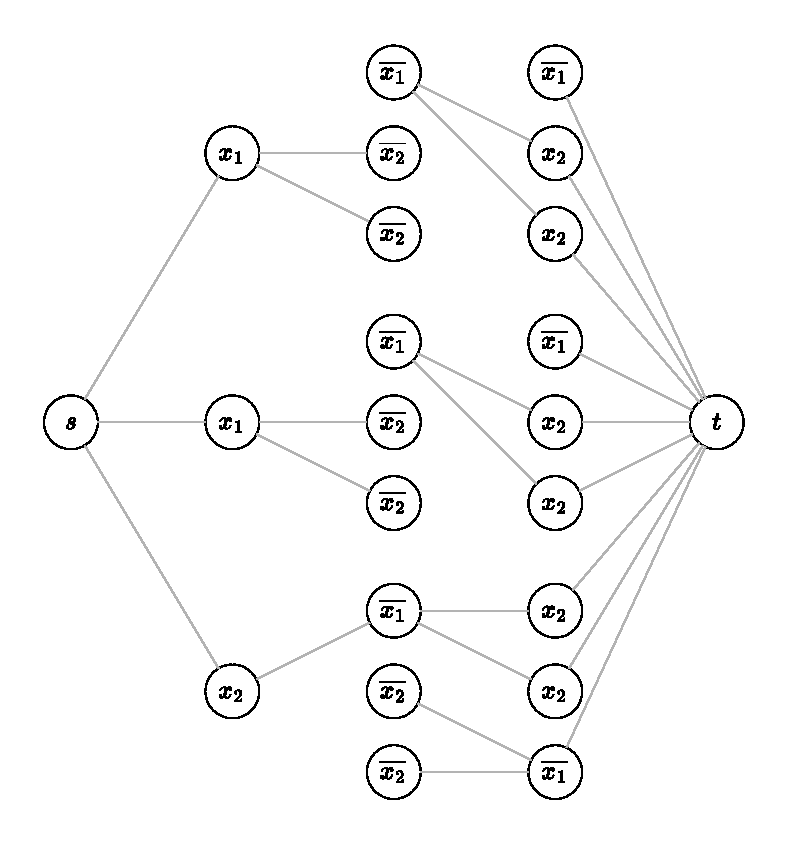
\includegraphics[scale=0.7]{Figures/Problem7.21.pdf} \\
Graph $G$ with $k=4$ for \\
$\phi = (x_1 \vee x_1 \vee x_2) \ \wedge (\overline{x_1} \vee \overline{x_2} \vee \overline{x_2}) \ \wedge (\overline{x_1} \vee x_2 \vee x_2)$.
\end{center}

\end{proof}

\end{document}